\subsection{Handling categorical features}

So far we assumed features (both descriptive and target) are continuous. In this chapter, we'll look at categorical descriptive and target features.
\begin{note}
  \begin{itemize}
    \item E.g., $\{$true, false$\}$, $\{$A, B, C$\}$, or similar
  \end{itemize}
\end{note}

For \textbf{categorical descriptive features}, we'll introduce $\{0$, $1\}$-features for every possible value, which is called \textbf{one hot encoding}\sidenote{One hot encoding}.
\begin{note}
  \begin{itemize}
    \item E.g., for $\{$A, B, C$\}$: A$=(1,0,0)$, B$=(0,1,0)$, C$=(0,0,1)$
  \end{itemize}
\end{note}

Next to one hot encoding, we have \textbf{single numeric value encoding}:
\begin{itemize}
  \item Binary values $\{$true, false$\}$ which can be translated to $\{$0, 1$\}$.
  \item Also, categorical variables with a clear order (ordinal) like $\{$good, average, poor$\}$ can be translated to $\{$$1.0$, $0.5$, $0.0$$\}$.
\end{itemize}

Possible issues are:
\begin{itemize}
  \item Adding order to unordered categorical variables resulting in nonsense
  \begin{note}
    \begin{itemize}
      \item E.g., simple encoding applied to country names maps numbers to countries (but no natural order exists)
    \end{itemize}
  \end{note}
  \item All encodings are approximations, so intermediate values will be considered possible by the "regression machine"
  \item One hot encoding discards dependencies
  \begin{itemize}
    \item Say if A$=1$ then logically B$=0$, but B$=0.66$ is also possible
  \end{itemize}
  \item Approach may introduce many additional features, making the problem computationally expensive
\end{itemize}

For a \textbf{categorical target feature} we can try to derive a numerical (continuous) feature. The naive approach is to find a line separating the results (try to find a line s.t. $\mathbf{w}\mathbf{d}=0$). The line then performs more of a separation than a prediction.

\begin{figure}[H]
  \centering
  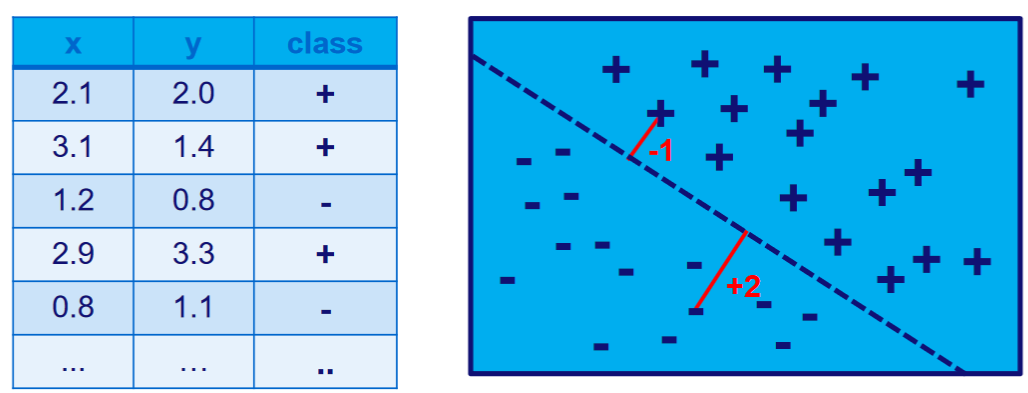
\includegraphics[width=0.6\textwidth]{assets/regression/cf__target_line.png}

  Target feature is +/- label, and not the value on the y-axis
  \caption{Seperating target feature (alternative to prediction)}
  \label{fig:4_cat_target_line}
\end{figure}

This means, we can use the $\{0, 1\}$ idea for encoding the two catgories (+/-). The model then also produces either 0 or 1:
\begin{align*}\begin{aligned}
  \mathbb{M}_\mathbf{w}(\mathbf{d})=\left\{ \begin{array}{ll}1&\text{if }\mathbf{w}\cdot\mathbf{d}\geq0\\ 0 &\text{else}\end{array} \right.
\end{aligned}\end{align*}

After this step, do business as usual e.g. by minimizing the sum of squared errors.
\begin{itemize}
  \item Notice that in this naive approach, we don't use the distance to the decision boundary yet.
  \item But this would be desirable to make the decision surface continuous or smooth and thereby more applicable to gradient descent.
\end{itemize}